% ============================================================
%  Chapter 6: Second-Order Methods
%  Algorithms for Optimization, 2nd ed. (2026)
%  Kochenderfer & Wheeler
%  Beamer slides – self-contained, Python examples
% ============================================================
\documentclass[aspectratio=169,10pt]{beamer}

\usetheme{Madrid}
\usecolortheme{seahorse}

\usepackage{amsmath,amssymb,bm}
\usepackage{mathtools}
\usepackage{graphicx}
\usepackage{booktabs}
\usepackage{listings}
\usepackage{xcolor}
\usepackage{tikz}
\usetikzlibrary{arrows.meta,positioning,shapes.geometric}
\usepackage{algorithm}
\usepackage{algpseudocode}

\graphicspath{{figures/}}

\setbeamertemplate{footline}[frame number]
\setbeamertemplate{navigation symbols}{}

% ── Python listings style ─────────────────────────────────────
\lstdefinestyle{pycode}{
  language=Python,
  basicstyle=\ttfamily\scriptsize,
  keywordstyle=\color{blue!70!black}\bfseries,
  commentstyle=\color{gray!70},
  stringstyle=\color{orange!80!black},
  numbers=left,
  numberstyle=\tiny\color{gray},
  stepnumber=1,
  numbersep=5pt,
  frame=single,
  backgroundcolor=\color{gray!7},
  breaklines=true,
  showstringspaces=false,
  tabsize=4,
}
\lstset{style=pycode}

% ── Convenience macros ────────────────────────────────────────
\newcommand{\xbf}{\mathbf{x}}
\newcommand{\gbf}{\mathbf{g}}
\newcommand{\Hbf}{\mathbf{H}}
\newcommand{\Ibf}{\mathbf{I}}
\newcommand{\R}{\mathbb{R}}
\newcommand{\deltabf}{\boldsymbol{\delta}}
\newcommand{\gammabf}{\boldsymbol{\gamma}}
\DeclareMathOperator*{\argmin}{arg\,min}

% ──────────────────────────────────────────────────────────────
\title[Ch.\,6 Second-Order Methods]{Chapter 6: Second-Order Methods}
\subtitle{Algorithms for Optimization, 2\textsuperscript{nd} ed.\ (2026)}
\author{Kochenderfer \& Wheeler}
\institute{Lecture Slides}
\date{}
% ──────────────────────────────────────────────────────────────

\begin{document}

% ── Title slide ───────────────────────────────────────────────
\begin{frame}
  \titlepage
\end{frame}

% ── Outline ───────────────────────────────────────────────────
\begin{frame}{Outline}
  \tableofcontents
\end{frame}

% ══════════════════════════════════════════════════════════════
\section{Introduction}
% ══════════════════════════════════════════════════════════════

\begin{frame}{Motivation: Why Second-Order Information?}
  \begin{columns}[T]
    \begin{column}{0.55\textwidth}
      \begin{block}{First-Order Methods}
        \begin{itemize}
          \item Use gradient $\nabla f(\xbf)$ to determine direction
          \item Do \emph{not} directly inform the step size needed to reach a minimum
          \item Can take many small steps in curved regions
        \end{itemize}
      \end{block}
      \vspace{4pt}
      \begin{block}{Second-Order Methods}
        \begin{itemize}
          \item Use the Hessian $\mathbf{H}(\xbf) = \nabla^2 f(\xbf)$
          \item Build a \emph{quadratic} local model of $f$
          \item Quadratic models have an analytically optimal step
          \item Can converge in a single step on quadratic functions
        \end{itemize}
      \end{block}
      \vspace{4pt}
      \begin{alertblock}{Key Idea}
        A bowl-shaped quadratic approximation has a unique point
        where the derivative is zero --- jump there directly!
      \end{alertblock}
    \end{column}
    \begin{column}{0.42\textwidth}
      \centering
      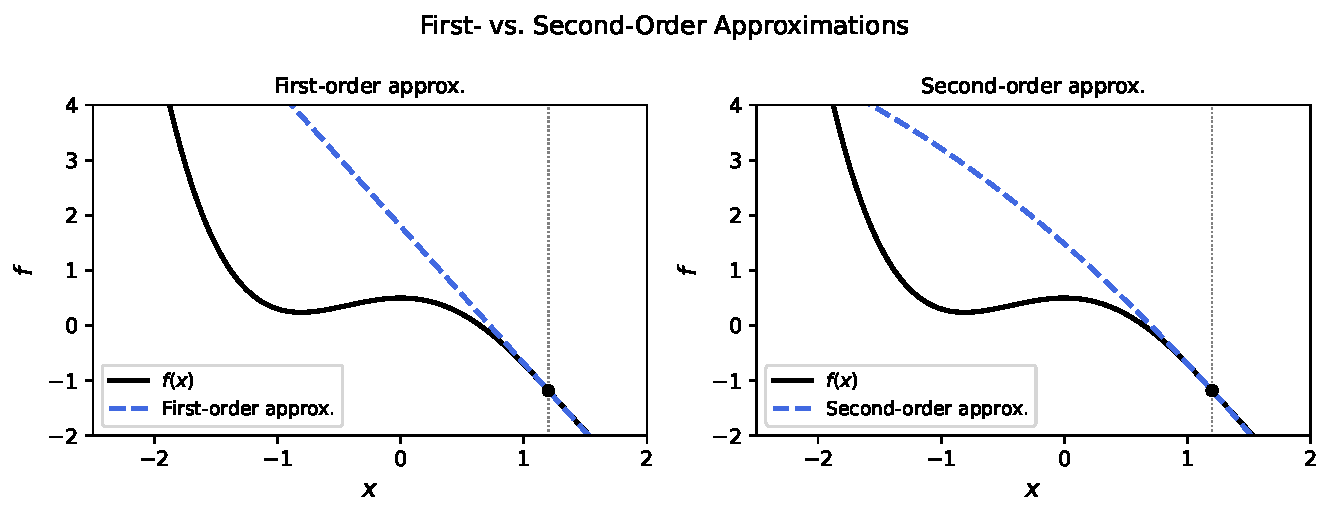
\includegraphics[width=\textwidth]{fig_first_vs_second_order.pdf}
      \\[4pt]
      {\scriptsize Top: first-order (linear) approx.\ misses the minimum.
       Bottom: second-order (quadratic) approx.\ locates the minimum.}
    \end{column}
  \end{columns}
\end{frame}

\begin{frame}{Quadratic Approximation (Taylor Expansion)}
  \begin{block}{Univariate: Second-Order Taylor Expansion (Eq.\ 6.1)}
    \[
      q(x) = f\!\left(x^{(k)}\right) + \bigl(x - x^{(k)}\bigr)f'\!\left(x^{(k)}\right)
             + \frac{\bigl(x - x^{(k)}\bigr)^2}{2}\,f''\!\left(x^{(k)}\right)
    \]
    \smallskip
    \begin{itemize}
      \item $x^{(k)}$ -- current iterate (expansion point)
      \item $f'(x^{(k)})$ -- first derivative (slope) at $x^{(k)}$
      \item $f''(x^{(k)})$ -- second derivative (curvature) at $x^{(k)}$
    \end{itemize}
  \end{block}

  \begin{block}{Multivariate: Second-Order Taylor Expansion}
    \[
      q(\xbf) = f(\xbf^{(k)}) + \bigl(\xbf - \xbf^{(k)}\bigr)^\top \gbf^{(k)}
                + \tfrac{1}{2}\bigl(\xbf - \xbf^{(k)}\bigr)^\top \Hbf^{(k)}\bigl(\xbf - \xbf^{(k)}\bigr)
    \]
    \begin{itemize}
      \item $\gbf^{(k)} = \nabla f(\xbf^{(k)}) \in \R^n$ -- gradient vector
      \item $\Hbf^{(k)} = \nabla^2 f(\xbf^{(k)}) \in \R^{n\times n}$ -- Hessian matrix
    \end{itemize}
  \end{block}
  \vspace{2pt}
  Setting $\nabla q(\xbf) = 0$ gives the Newton step directly.
\end{frame}

% ══════════════════════════════════════════════════════════════
\section{Newton's Method}
% ══════════════════════════════════════════════════════════════

\begin{frame}{6.1 Newton's Method}
  \begin{block}{Univariate Update Rule (Eq.\ 6.3--6.4)}
    Setting $q'(x) = 0$ and solving for the next iterate:
    \[
      x^{(k+1)} \leftarrow x^{(k)} - \frac{f'(x^{(k)})}{f''(x^{(k)})}
    \]
  \end{block}

  \begin{block}{Multivariate Update Rule (Eq.\ 6.6)}
    Setting $\nabla q(\xbf) = 0$ and solving for $\xbf$:
    \[
      \xbf^{(k+1)} \leftarrow \xbf^{(k)} - \left(\Hbf^{(k)}\right)^{-1} \gbf^{(k)}
    \]
    \begin{itemize}
      \item $\gbf^{(k)} = \nabla f(\xbf^{(k)})$ -- gradient at current iterate
      \item $\Hbf^{(k)} = \nabla^2 f(\xbf^{(k)})$ -- Hessian at current iterate
      \item In practice: solve $\Hbf^{(k)}\,\mathbf{d} = -\gbf^{(k)}$, then $\xbf^{(k+1)} = \xbf^{(k)} + \mathbf{d}$
    \end{itemize}
  \end{block}

  \begin{alertblock}{Descent Direction}
    The Newton direction $\mathbf{d} = -(\Hbf^{(k)})^{-1}\gbf^{(k)}$ is a
    descent direction when $\Hbf^{(k)}$ is \emph{positive definite}.
  \end{alertblock}
\end{frame}

\begin{frame}[allowframebreaks]{Newton's Method: Algorithm \& Convergence}
  \begin{block}{Algorithm 6.1: Newton's Method}
    \begin{enumerate}
      \item \textbf{Input:} $f$, $f'$/$\nabla f$, $f''$/$\nabla^2 f$, initial $\xbf^{(1)}$, tolerance $\epsilon$
      \item \textbf{Repeat} until $\|\gbf^{(k)}\| \leq \epsilon$:
      \begin{enumerate}
        \item Compute $\gbf^{(k)} = \nabla f(\xbf^{(k)})$
        \item Compute $\Hbf^{(k)} = \nabla^2 f(\xbf^{(k)})$
        \item Solve $\Hbf^{(k)}\mathbf{d} = -\gbf^{(k)}$
        \item Update: $\xbf^{(k+1)} \leftarrow \xbf^{(k)} + \mathbf{d}$
      \end{enumerate}
      \item \textbf{Return} $\xbf^{(k+1)}$
    \end{enumerate}
  \end{block}

  \begin{block}{Convergence Properties}
    \begin{itemize}
      \item \textbf{Quadratic convergence} near a local minimum (error squares at each step)
      \item Converges in \textbf{one step} on strictly quadratic functions
      \item Often terminated once $x^{(k+1)}$ changes by less than some tolerance $\epsilon$
      \item \textbf{Cost per iteration:} $O(n^3)$ for Hessian inversion (or $O(n^2)$ with structure)
    \end{itemize}
  \end{block}

  \framebreak

  \begin{columns}[T]
    \begin{column}{0.50\textwidth}
      \begin{alertblock}{Potential Problems}
        \begin{itemize}
          \item $f''(x^{(k)}) = 0$ or $\Hbf^{(k)}$ singular: undefined step
          \item $f''(x^{(k)}) < 0$: step goes uphill (oscillation or divergence)
          \item Not guaranteed to descend: may need line search
          \item Requires second derivatives (costly to compute)
        \end{itemize}
      \end{alertblock}
    \end{column}
    \begin{column}{0.48\textwidth}
      \centering
      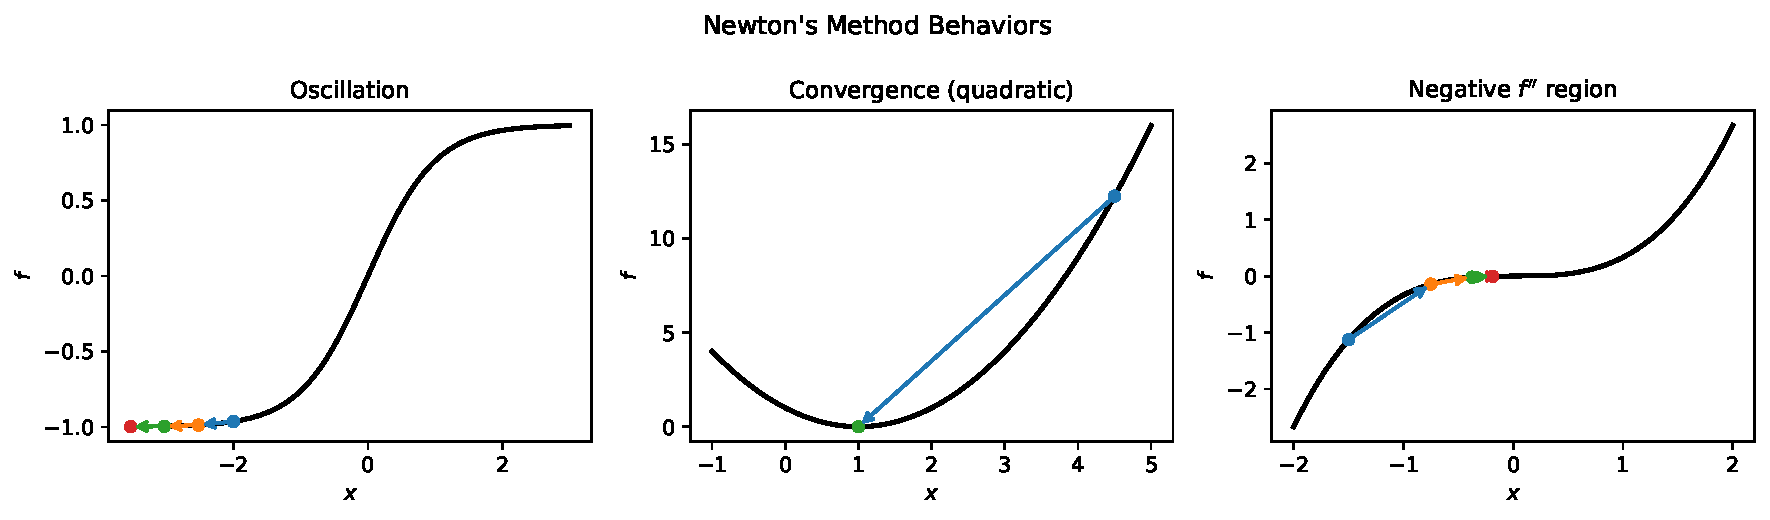
\includegraphics[width=\textwidth]{fig_newton_behaviors.pdf}
      {\scriptsize Oscillation (left), convergence (center), divergence near negative $f''$ (right)}
    \end{column}
  \end{columns}
\end{frame}

\begin{frame}{Newton's Method: Iterations on 1D Function}
  \begin{columns}[T]
    \begin{column}{0.48\textwidth}
      \centering
      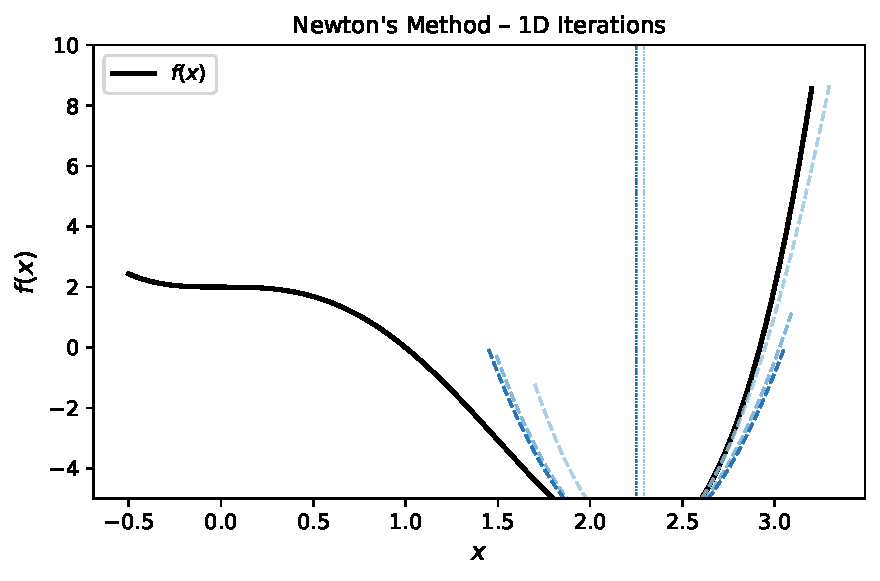
\includegraphics[width=\textwidth]{fig_newton_1d.pdf}
      {\scriptsize Quadratic approximations (dashed) converging to minimum.}
    \end{column}
    \begin{column}{0.50\textwidth}
      \begin{block}{Key Observations}
        \begin{itemize}
          \item Each dashed curve is the quadratic approximation $q(x)$ at the current point
          \item The next iterate is the minimum of $q(x)$
          \item Near the minimum, convergence is quadratic
          \item Far from minimum, behavior can be unpredictable
        \end{itemize}
      \end{block}
      \begin{block}{Termination Criteria}
        Terminate when \emph{any} of these are satisfied:
        \begin{enumerate}
          \item $\|\gbf^{(k)}\| \leq \epsilon$ (gradient small)
          \item $\|x^{(k+1)} - x^{(k)}\| \leq \epsilon$ (step small)
          \item Maximum iterations reached
        \end{enumerate}
      \end{block}
    \end{column}
  \end{columns}
\end{frame}

\begin{frame}[fragile]{Newton's Method: Python Implementation}
\begin{lstlisting}[caption={Newton's method (multivariate) in Python}]
import numpy as np
from numpy.linalg import solve, norm

def newtons_method(f, grad_f, hess_f, x0, eps=1e-8, max_iter=100):
    """
    Newton's method for unconstrained minimization.
    f       : objective function R^n -> R
    grad_f  : gradient function R^n -> R^n
    hess_f  : Hessian function  R^n -> R^{n x n}
    x0      : initial point (numpy array)
    """
    x = np.array(x0, dtype=float)
    history = [x.copy()]
    for k in range(max_iter):
        g = grad_f(x)
        if norm(g) < eps:
            break
        H = hess_f(x)
        # Solve H*d = -g  (more stable than inverting H)
        d = solve(H, -g)
        x = x + d
        history.append(x.copy())
    return x, history

# --- Example: Booth's function f(x) = (x1+2x2-7)^2 + (2x1+x2-5)^2 ---
def booth(x):
    return (x[0] + 2*x[1] - 7)**2 + (2*x[0] + x[1] - 5)**2

def grad_booth(x):
    return np.array([
        2*(x[0]+2*x[1]-7) + 4*(2*x[0]+x[1]-5),
        4*(x[0]+2*x[1]-7) + 2*(2*x[0]+x[1]-5)
    ])

def hess_booth(x):
    return np.array([[10., 8.], [8., 10.]])  # constant Hessian

x_opt, hist = newtons_method(booth, grad_booth, hess_booth, x0=[9., 8.])
print(f"Minimum at: {x_opt}")   # -> [1. 3.]
print(f"Iterations: {len(hist)-1}")  # -> 1 (one step!)
\end{lstlisting}
\end{frame}

\begin{frame}{Example 6.1: Newton's Method on Booth's Function}
  \begin{columns}[T]
    \begin{column}{0.52\textwidth}
      \begin{block}{Booth's Function}
        \[
          f(\xbf) = (x_1 + 2x_2 - 7)^2 + (2x_1 + x_2 - 5)^2
        \]
        Global minimum at $\xbf^* = [1,\,3]^\top$.
      \end{block}
      \begin{block}{Gradient}
        \[
          \nabla f(\xbf) = \begin{bmatrix}10x_1 + 8x_2 - 34\\8x_1 + 10x_2 - 38\end{bmatrix}
        \]
      \end{block}
      \begin{block}{Hessian (constant!)}
        \[
          \mathbf{H}(\xbf) = \begin{bmatrix}10 & 8\\8 & 10\end{bmatrix}
        \]
      \end{block}
    \end{column}
    \begin{column}{0.46\textwidth}
      \begin{block}{One Newton Step from $\xbf^{(1)} = [9,8]^\top$}
        \scriptsize
        \[
          \xbf^{(2)} = \begin{bmatrix}9\\8\end{bmatrix}
          - \begin{bmatrix}10&8\\8&10\end{bmatrix}^{-1}
            \begin{bmatrix}10\!\cdot\!9 + 8\!\cdot\!8 - 34\\8\!\cdot\!9 + 10\!\cdot\!8 - 38\end{bmatrix}
        \]
        \[
          = \begin{bmatrix}9\\8\end{bmatrix}
          - \begin{bmatrix}10&8\\8&10\end{bmatrix}^{-1}
            \begin{bmatrix}120\\114\end{bmatrix}
          = \begin{bmatrix}1\\3\end{bmatrix}
        \]
      \end{block}
      \begin{alertblock}{Result}
        Converged in \textbf{one iteration}! The Hessian is
        positive definite everywhere, so $\xbf^{(2)} = [1,3]^\top$
        is the global minimum.
      \end{alertblock}
      \centering
      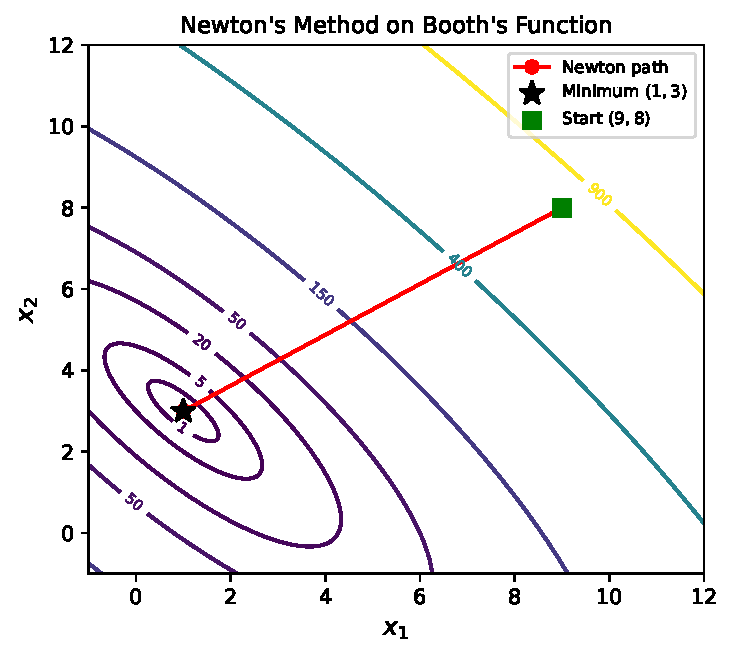
\includegraphics[width=0.85\textwidth]{fig_booth_newton.pdf}
    \end{column}
  \end{columns}
\end{frame}

% ══════════════════════════════════════════════════════════════
\section{Secant Method}
% ══════════════════════════════════════════════════════════════

\begin{frame}{6.2 Secant Method}
  \begin{columns}[T]
    \begin{column}{0.55\textwidth}
      \begin{block}{Motivation}
        Newton's method requires the second derivative $f''$.
        The \textbf{secant method} approximates $f''$ from two
        recent function evaluations.
      \end{block}

      \begin{block}{Second Derivative Approximation (Eq.\ 6.8)}
        \[
          f''\!\left(x^{(k)}\right) \approx
          \frac{f'\!\left(x^{(k)}\right) - f'\!\left(x^{(k-1)}\right)}
               {x^{(k)} - x^{(k-1)}}
        \]
      \end{block}

      \begin{block}{Secant Update Rule (Eq.\ 6.9)}
        Substituting into Newton's method:
        \[
          x^{(k+1)} \leftarrow x^{(k)} - \frac{x^{(k)} - x^{(k-1)}}
                                               {f'\!\left(x^{(k)}\right) - f'\!\left(x^{(k-1)}\right)}
                                         \, f'\!\left(x^{(k)}\right)
        \]
      \end{block}
    \end{column}
    \begin{column}{0.43\textwidth}
      \centering
      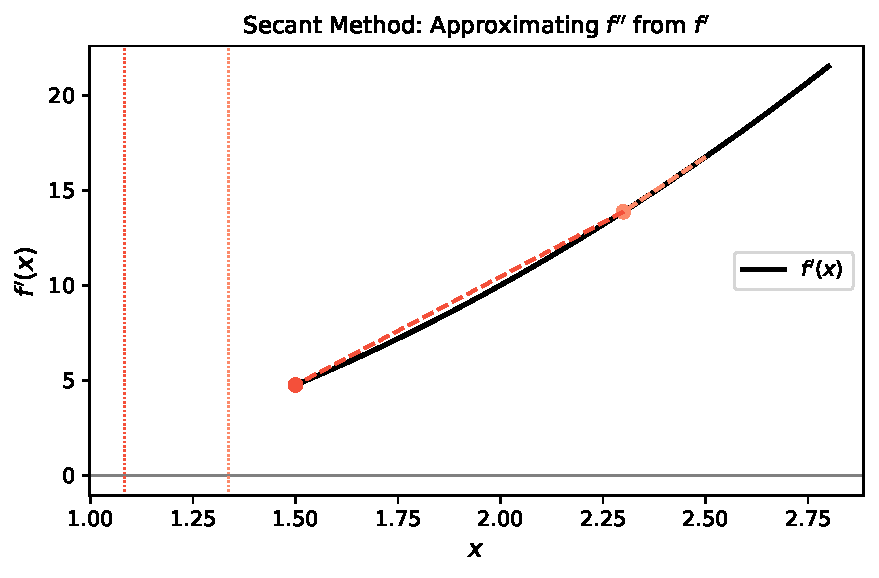
\includegraphics[width=\textwidth]{fig_secant_method.pdf}
      {\scriptsize The secant line through two evaluations of $f'$
       is used to approximate $f''$ and find the next iterate.}
    \end{column}
  \end{columns}
\end{frame}

\begin{frame}{Secant Method: Properties}
  \begin{columns}[T]
    \begin{column}{0.50\textwidth}
      \begin{block}{Algorithm 6.2: Secant Method}
        \begin{enumerate}
          \item \textbf{Input:} $f'$, initial $x^{(1)}$, step $\alpha$, tolerance $\epsilon$
          \item \textbf{Initialize:} $x_\text{prev} = x^{(1)} + \alpha f'(x^{(1)})$,
                $g_\text{prev} = f'(x_\text{prev})$
          \item \textbf{Repeat:}
          \begin{enumerate}
            \item $g \leftarrow f'(x)$
            \item $x' \leftarrow x - \dfrac{x - x_\text{prev}}{g - g_\text{prev}}\cdot g$
            \item $x_\text{prev}, g_\text{prev} \leftarrow x,\; g$
            \item $x \leftarrow x'$
          \end{enumerate}
        \end{enumerate}
      \end{block}
    \end{column}
    \begin{column}{0.48\textwidth}
      \begin{block}{Properties}
        \begin{itemize}
          \item Requires only \textbf{first derivative} $f'$
          \item Needs one extra initial point to start
          \item Suffers the same problems as Newton's method
            (oscillation, negative curvature)
          \item May take \textbf{more iterations} than Newton's
            due to approximate curvature
          \item \textbf{Superlinear convergence} (order $\approx 1.618$,
            the golden ratio)
        \end{itemize}
      \end{block}
      \begin{alertblock}{Univariate only}
        The secant method as stated applies to univariate
        objective functions. Quasi-Newton methods generalize
        this idea to multivariate problems.
      \end{alertblock}
    \end{column}
  \end{columns}
\end{frame}

\begin{frame}[fragile]{Secant Method: Python Implementation}
\begin{lstlisting}[caption={Secant method for univariate minimization in Python}]
import numpy as np

def secant_method(fp, x0, alpha=1e-3, eps=1e-8, max_iter=200):
    """
    Secant method for univariate minimization.
    fp  : first derivative f'(x)
    x0  : initial point
    alpha: step for initializing previous point
    """
    x_prev = x0 + alpha * fp(x0)  # small step in gradient direction
    g_prev = fp(x_prev)
    x = x0
    history = [x]

    for _ in range(max_iter):
        g = fp(x)
        if abs(g) < eps:
            break
        denom = g - g_prev
        if abs(denom) < 1e-14:
            break                        # avoid division by zero
        x_new = x - (x - x_prev) / denom * g
        x_prev, g_prev = x, g
        x = x_new
        history.append(x)

    return x, history

# Example: minimize f(x) = x^4 - 3x^3 + 2,  f'(x) = 4x^3 - 9x^2
fp = lambda x: 4*x**3 - 9*x**2
x_min, hist = secant_method(fp, x0=3.0)
print(f"Minimum at x = {x_min:.6f}")    # ~2.25 (local min)
print(f"Iterations:   {len(hist)-1}")
\end{lstlisting}
\end{frame}

% ══════════════════════════════════════════════════════════════
\section{Levenberg-Marquardt Algorithm}
% ══════════════════════════════════════════════════════════════

\begin{frame}{6.3 Levenberg-Marquardt Algorithm}
  \begin{columns}[T]
    \begin{column}{0.55\textwidth}
      \begin{block}{Motivation}
        Newton's method uses
        $\xbf^{(k+1)} = \xbf^{(k)} - \Hbf^{-1}\gbf$,
        which can fail when:
        \begin{itemize}
          \item $\Hbf$ is indefinite or singular
          \item The quadratic approximation is poor (far from minimum)
        \end{itemize}
        \textbf{Idea:} Interpolate between gradient descent and Newton.
      \end{block}

      \begin{block}{LM Update -- Plain Damping (Eq.\ 6.10)}
        \[
          \xbf^{(k+1)} = \xbf^{(k)} - \left(\Hbf^{(k)} + \delta\Ibf\right)^{-1}\gbf^{(k)}
        \]
        \begin{itemize}
          \item Small $\delta$: approaches Newton's step
          \item Large $\delta$: approaches gradient descent
        \end{itemize}
      \end{block}

      \begin{block}{LM Update -- Diagonal Scaling (Eq.\ 6.11)}
        \[
          \xbf^{(k+1)} = \xbf^{(k)} - \left(\Hbf^{(k)} + \delta\,\mathrm{diag}(\Hbf^{(k)})\right)^{-1}\gbf^{(k)}
        \]
        Scales the damping relative to the local curvature.
      \end{block}
    \end{column}
    \begin{column}{0.43\textwidth}
      \centering
      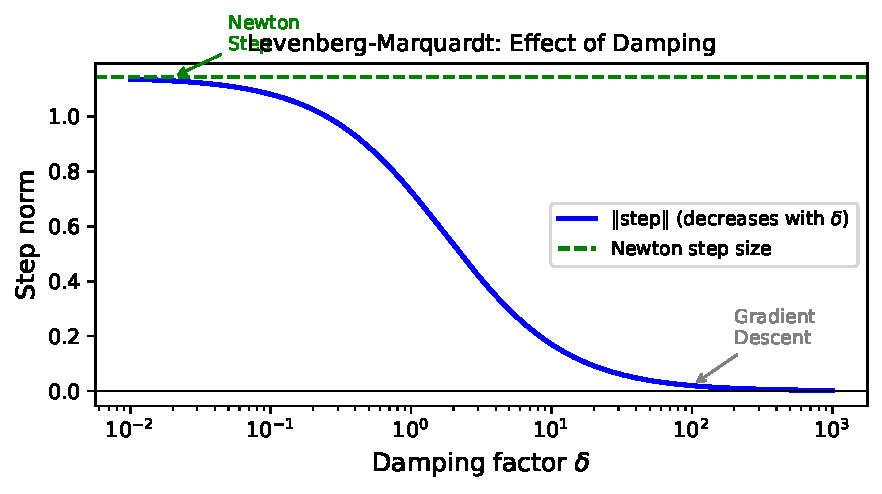
\includegraphics[width=\textwidth]{fig_lm_damping.pdf}
      {\scriptsize As damping $\delta$ grows, the step shrinks from Newton size toward zero. Large $\delta$ gives gradient descent behavior.}
    \end{column}
  \end{columns}
\end{frame}

\begin{frame}[allowframebreaks]{LM Algorithm: Adaptive Damping}
  \begin{block}{Algorithm 6.3: Levenberg-Marquardt (Eq.\ 6.10/6.11)}
    \textbf{Input:} $f$, $\nabla f$, $\Hbf$, $\xbf^{(1)}$, $\delta > 0$, $\gamma_\text{acc}$, $\gamma_\text{rej}$, $\epsilon$
    \begin{enumerate}
      \item Compute $\Hbf = \Hbf(\xbf)$, $\gbf = \nabla f(\xbf)$
      \item Form damped matrix: $\mathbf{M} = \Hbf + \delta\,\mathrm{diag}\!\left(\max(\mathrm{diag}(\Hbf),\,\epsilon)\right)$
      \item Compute candidate: $\xbf' = \xbf - \mathbf{M}^{-1}\gbf$
      \item \textbf{If} $f(\xbf') < f(\xbf)$ \textbf{(accept step):}
        \begin{itemize}
          \item $\xbf \leftarrow \xbf'$
          \item $\delta \leftarrow \delta \cdot \gamma_\text{acc}$ \quad (reduce damping)
        \end{itemize}
      \item \textbf{Else (reject step):}
        \begin{itemize}
          \item Keep $\xbf$ unchanged
          \item $\delta \leftarrow \delta \cdot \gamma_\text{rej}$ \quad (increase damping)
        \end{itemize}
      \item Repeat until convergence
    \end{enumerate}
  \end{block}

  \begin{block}{Parameter Guidelines}
    \begin{tabular}{lll}
      \toprule
      Parameter & Meaning & Typical value \\
      \midrule
      $\delta$ & initial damping factor & $1.0$ \\
      $\gamma_\text{acc}$ & damping decrease factor (accept) & $0.1$ \\
      $\gamma_\text{rej}$ & damping increase factor (reject) & $10.0$ \\
      $\epsilon$ & floor for diagonal elements & $10^{-6}$ \\
      \bottomrule
    \end{tabular}
  \end{block}

  \framebreak

  \begin{columns}[T]
    \begin{column}{0.50\textwidth}
      \centering
      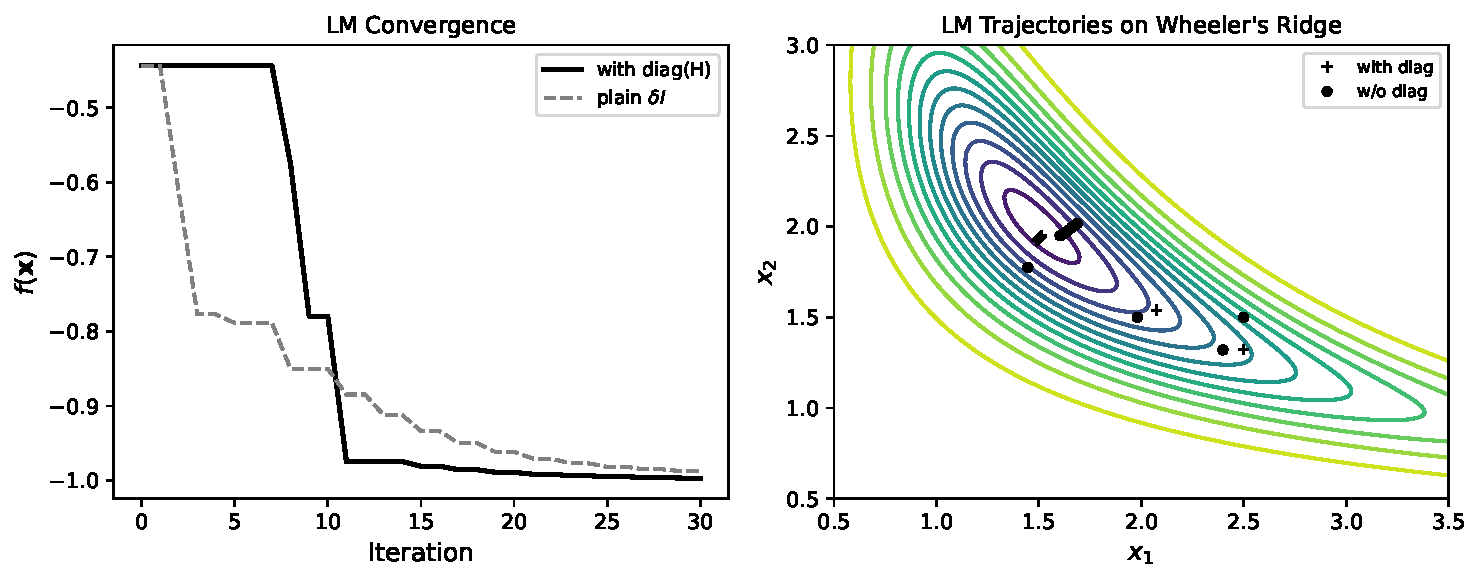
\includegraphics[width=\textwidth]{fig_lm_convergence.pdf}
      {\scriptsize LM convergence (left) and trajectories on Wheeler's Ridge (right).
       The variant with diagonal Hessian scaling converges more efficiently.}
    \end{column}
    \begin{column}{0.48\textwidth}
      \begin{block}{Why Diagonal Scaling Helps}
        \begin{itemize}
          \item Plain damping: adds $\delta\Ibf$ uniformly
          \item Diagonal: adds $\delta\,\mathrm{diag}(\Hbf)$, which is
            larger where curvature is larger
          \item Better scale-invariant behavior in flat regions
          \item Component-wise max with $\epsilon$ ensures the
            matrix is always invertible
        \end{itemize}
      \end{block}
    \end{column}
  \end{columns}
\end{frame}

\begin{frame}[fragile]{Levenberg-Marquardt: Python Implementation}
\begin{lstlisting}[caption={Levenberg-Marquardt algorithm in Python (NumPy)}]
import numpy as np
from numpy.linalg import solve

def levenberg_marquardt(f, grad_f, hess_f, x0,
                        delta=1.0, gamma_acc=0.1, gamma_rej=10.0,
                        eps=1e-6, max_iter=100):
    x = np.array(x0, dtype=float)
    history = [x.copy()]
    for _ in range(max_iter):
        g = grad_f(x)
        if np.linalg.norm(g) < eps:
            break
        H = hess_f(x)
        # Diagonal scaling: take component-wise max with eps
        d = np.maximum(np.diag(H), eps)
        M = H + delta * np.diag(d)
        try:
            step = solve(M, g)
        except np.linalg.LinAlgError:
            step = g   # fallback: gradient step
        x_new = x - step
        if f(x_new) < f(x):
            x = x_new
            delta *= gamma_acc          # accept: reduce damping
        else:
            delta *= gamma_rej          # reject: increase damping
        history.append(x.copy())
    return x, history
\end{lstlisting}
\end{frame}

% ══════════════════════════════════════════════════════════════
\section{Levenberg-Marquardt for Sum of Squares}
% ══════════════════════════════════════════════════════════════

\begin{frame}{6.4 LM for Sum of Squares}
  \begin{columns}[T]
    \begin{column}{0.55\textwidth}
      \begin{block}{Objective Function (Eq.\ 6.12)}
        \[
          f(\xbf) = \sum_i f_i(\xbf)^2
        \]
        Each $f_i : \R^n \to \R$ is a \emph{residual} function.
      \end{block}

      \begin{block}{Gradient (Eq.\ 6.13)}
        \[
          \nabla f(\xbf) = 2\sum_i f_i(\xbf)\,\nabla f_i(\xbf)
        \]
      \end{block}

      \begin{block}{Linear Approximation of Residuals (Eq.\ 6.14)}
        \[
          f_i(\xbf) \approx f_i\!\left(\xbf^{(k)}\right)
            + \nabla f_i\!\left(\xbf^{(k)}\right)^\top\!\bigl(\xbf - \xbf^{(k)}\bigr)
        \]
        Substituting into the gradient yields an approximate gradient
        of the form (Eq.\ 6.17):
        \[
          \nabla f(\xbf) \approx 2\tilde{\gbf}^{(k)} + 2\tilde{\Hbf}^{(k)}\bigl(\xbf - \xbf^{(k)}\bigr)
        \]
      \end{block}
    \end{column}
    \begin{column}{0.43\textwidth}
      \begin{block}{Outer Product Hessian Approximation}
        \begin{align*}
          \tilde{\gbf}^{(k)} &= \sum_i f_i(\xbf^{(k)})\,\nabla f_i(\xbf^{(k)}) \tag{6.18}\\[4pt]
          \tilde{\Hbf}^{(k)} &= \sum_i \nabla f_i(\xbf^{(k)})\,\nabla f_i(\xbf^{(k)})^\top \tag{6.19}
        \end{align*}
        Note: $\tilde{\Hbf}^{(k)}$ is the \textbf{Gauss-Newton} approximation
        (outer product of Jacobian rows), always \emph{positive semi-definite}.
      \end{block}
      \begin{alertblock}{Key Advantage}
        No need to compute true second derivatives!
        Only first derivatives $\nabla f_i$ are required.
      \end{alertblock}
    \end{column}
  \end{columns}
\end{frame}

\begin{frame}{LM Sum-of-Squares: Update Formula}
  \begin{block}{LM Update for Sum of Squares (Eq.\ 6.21)}
    Setting $\nabla f(\xbf) \approx 0$ and incorporating damping:
    \[
      \xbf^{(k+1)} = \xbf^{(k)}
        - \Bigl(\tilde{\Hbf}^{(k)} + \delta\,\mathrm{diag}\!\bigl(\tilde{\Hbf}^{(k)}\bigr)\Bigr)^{-1}
          \tilde{\gbf}^{(k)}
    \]
    \begin{itemize}
      \item $\tilde{\gbf}^{(k)} = \mathbf{J}^\top \mathbf{r}$ \quad (Jacobian times residual vector)
      \item $\tilde{\Hbf}^{(k)} = \mathbf{J}^\top \mathbf{J}$ \quad (Gauss-Newton Hessian, always $\succeq 0$)
      \item $\mathbf{J}_{ij} = \partial f_i / \partial x_j$ \quad (Jacobian matrix)
      \item $\mathbf{r}_i = f_i(\xbf)$ \quad (residual vector)
    \end{itemize}
  \end{block}

  \begin{columns}[T]
    \begin{column}{0.50\textwidth}
      \centering
      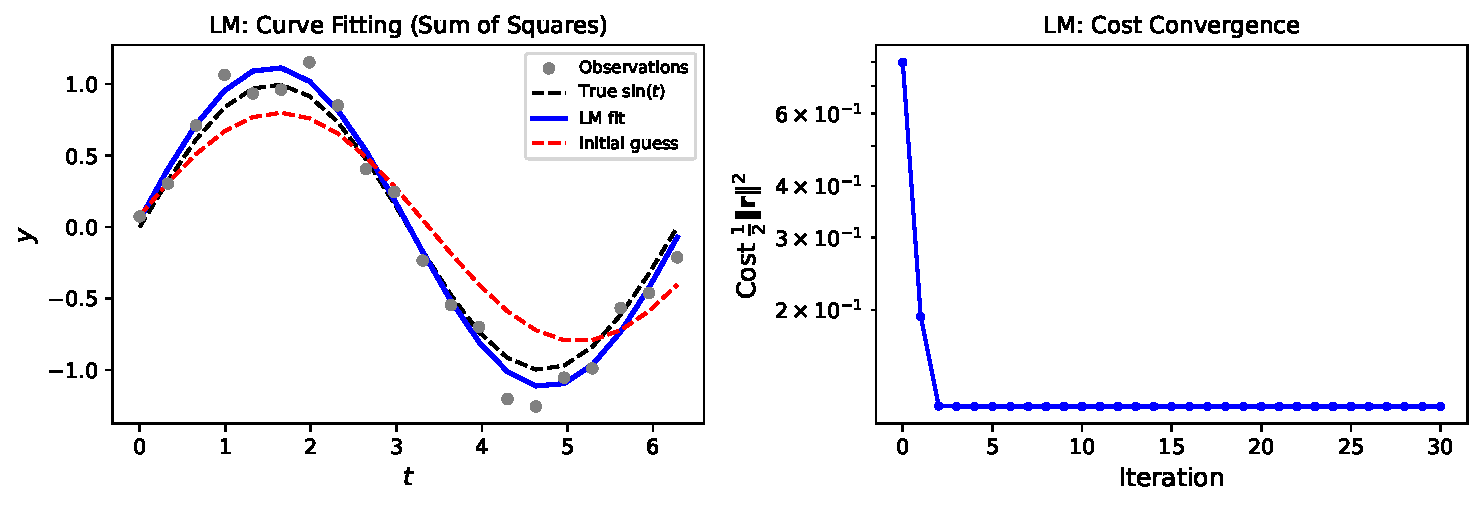
\includegraphics[width=\textwidth]{fig_lm_least_squares.pdf}
      {\scriptsize LM fitting $a\sin(bt+c)$ to noisy observations (left)
       and cost convergence (right).}
    \end{column}
    \begin{column}{0.48\textwidth}
      \begin{block}{Comparison: LM vs.\ Full Newton}
        \begin{tabular}{lcc}
          \toprule
          & LM (sum-of-sq) & Full Newton \\
          \midrule
          Hessian approx & $\mathbf{J}^\top\mathbf{J}$ & exact \\
          Always PSD? & \checkmark & No \\
          Cost/iter & $O(mn^2)$ & $O(n^3)$ \\
          Requires & $\mathbf{J}$ only & $\mathbf{J},\mathbf{H}$ \\
          \bottomrule
        \end{tabular}
        {\scriptsize $m$ = number of residuals, $n$ = problem dimension}
      \end{block}
    \end{column}
  \end{columns}
\end{frame}

\begin{frame}[fragile]{LM for Sum of Squares: Python with SciPy}
\begin{lstlisting}[caption={LM for nonlinear least squares using scipy.optimize.least\_squares}]
import numpy as np
from scipy.optimize import least_squares

# --- Curve fitting: model a*sin(b*t + c) ---
np.random.seed(42)
t_obs = np.linspace(0, 2*np.pi, 20)
y_obs = np.sin(t_obs) + 0.15 * np.random.randn(len(t_obs))

def model(params, t):
    a, b, c = params
    return a * np.sin(b * t + c)

def residuals(params):
    return model(params, t_obs) - y_obs  # vector of f_i(x)

# SciPy uses LM (method='lm') or trust-region approaches
result = least_squares(residuals, x0=[0.8, 0.9, 0.1], method='lm')

print(f"Fitted params:   a={result.x[0]:.4f}, b={result.x[1]:.4f}, c={result.x[2]:.4f}")
print(f"True params:     a=1.0000, b=1.0000, c=0.0000")
print(f"Final residual:  {0.5 * result.cost:.6f}")
print(f"Function evals:  {result.nfev}")

# Manual approach: build Jacobian explicitly
def jacobian(params, t):
    a, b, c = params
    dfa = np.sin(b*t + c)           # df/da
    dfb = a * t * np.cos(b*t + c)   # df/db
    dfc = a * np.cos(b*t + c)       # df/dc
    return np.column_stack([dfa, dfb, dfc])  # shape (m, 3)

J = jacobian(result.x, t_obs)
H_approx = J.T @ J                  # Gauss-Newton Hessian (3x3)
g_approx = J.T @ residuals(result.x)
print(f"\nGauss-Newton gradient norm: {np.linalg.norm(g_approx):.2e}")
\end{lstlisting}
\end{frame}

% ══════════════════════════════════════════════════════════════
\section{Quasi-Newton Methods}
% ══════════════════════════════════════════════════════════════

\begin{frame}{6.5 Quasi-Newton Methods: Overview}
  \begin{block}{Motivation}
    Computing the full Hessian $\Hbf^{(k)}$ at each iteration costs $O(n^2)$ evaluations
    and $O(n^3)$ to invert. \textbf{Quasi-Newton methods} approximate the inverse
    Hessian $\mathbf{Q}^{(k)} \approx \left(\Hbf^{(k)}\right)^{-1}$ using only gradient
    information.
  \end{block}

  \begin{block}{General Quasi-Newton Update}
    \[
      \xbf^{(k+1)} = \xbf^{(k)} - \mathbf{Q}^{(k)}\,\gbf^{(k)}
    \]
    $\mathbf{Q}^{(k)}$ is updated at each step using the \textbf{secant condition}:
    \[
      \mathbf{Q}^{(k+1)}\,\deltabf^{(k)} = \gammabf^{(k)}
    \]
    where:
    \begin{itemize}
      \item $\deltabf^{(k)} = \xbf^{(k+1)} - \xbf^{(k)}$ \quad (step vector)
      \item $\gammabf^{(k)} = \gbf^{(k+1)} - \gbf^{(k)}$ \quad (gradient difference)
    \end{itemize}
  \end{block}

  \begin{block}{Three Variants}
    \centering
    \begin{tabular}{lll}
      \toprule
      Method & Rank-update & Memory \\
      \midrule
      SR1  & rank-1 & $O(n^2)$ \\
      DFP  & rank-2 & $O(n^2)$ \\
      BFGS & rank-2 (better) & $O(n^2)$ \\
      L-BFGS & limited-memory & $O(mn)$ \\
      \bottomrule
    \end{tabular}
  \end{block}
\end{frame}

\begin{frame}{DFP Update (Algorithm 6.5)}
  \begin{block}{Davidon-Fletcher-Powell Update}
    \[
      \mathbf{Q}^{(k+1)} = \mathbf{Q}^{(k)}
        - \frac{\mathbf{Q}^{(k)}\gammabf\,\gammabf^\top \mathbf{Q}^{(k)}}
               {\gammabf^\top \mathbf{Q}^{(k)}\gammabf}
        + \frac{\deltabf\,\deltabf^\top}{\deltabf^\top\gammabf}
    \]
    where $\deltabf = \xbf^{(k+1)} - \xbf^{(k)}$ and $\gammabf = \gbf^{(k+1)} - \gbf^{(k)}$.
  \end{block}

  \begin{columns}[T]
    \begin{column}{0.50\textwidth}
      \begin{block}{DFP Algorithm Steps}
        \begin{enumerate}
          \item Initialize $\mathbf{Q}^{(1)} = \Ibf_n$
          \item $\mathbf{d}^{(k)} = -\mathbf{Q}^{(k)}\gbf^{(k)}$
          \item Line search: $\alpha^* = \argmin_\alpha f(\xbf^{(k)} + \alpha\mathbf{d}^{(k)})$
          \item $\xbf^{(k+1)} = \xbf^{(k)} + \alpha^*\mathbf{d}^{(k)}$
          \item $\deltabf = \xbf^{(k+1)} - \xbf^{(k)}$,
                $\gammabf = \gbf^{(k+1)} - \gbf^{(k)}$
          \item Update $\mathbf{Q}^{(k+1)}$ via DFP formula
        \end{enumerate}
      \end{block}
    \end{column}
    \begin{column}{0.48\textwidth}
      \begin{block}{Properties}
        \begin{itemize}
          \item Maintains $\mathbf{Q} \succ 0$ (positive definite) if
            $\deltabf^\top\gammabf > 0$ (curvature condition)
          \item Enforces the secant equation:
            $\mathbf{Q}^{(k+1)}\gammabf = \deltabf$
          \item Rank-2 update (adds two rank-1 matrices)
          \item Works well with \emph{exact} line search
          \item DFP can underperform with inexact line search
        \end{itemize}
      \end{block}
    \end{column}
  \end{columns}
\end{frame}

\begin{frame}{BFGS Update (Algorithm 6.6)}
  \begin{block}{Broyden-Fletcher-Goldfarb-Shanno Update (Eq.\ 6.25)}
    \[
      \mathbf{Q}^{(k+1)} =
        \left(\Ibf - \rho\,\deltabf\,\gammabf^\top\right)
        \mathbf{Q}^{(k)}
        \left(\Ibf - \rho\,\gammabf\,\deltabf^\top\right)
        + \rho\,\deltabf\,\deltabf^\top
    \]
    where $\rho = \dfrac{1}{\deltabf^\top\gammabf}$.
  \end{block}

  \begin{columns}[T]
    \begin{column}{0.50\textwidth}
      \begin{block}{Why BFGS $>$ DFP?}
        \begin{itemize}
          \item BFGS is the \emph{dual} of DFP (swap roles of
            $\deltabf$ and $\gammabf$)
          \item More robust with \textbf{inexact} line search
          \item Both are rank-2 updates
          \item BFGS has better numerical properties in practice
          \item One of the most widely used optimization algorithms
        \end{itemize}
      \end{block}
      \begin{alertblock}{Update skipped when}
        $\deltabf^\top\gammabf \approx 0$ (curvature condition violated);
        simply skip the update in that iteration.
      \end{alertblock}
    \end{column}
    \begin{column}{0.48\textwidth}
      \centering
      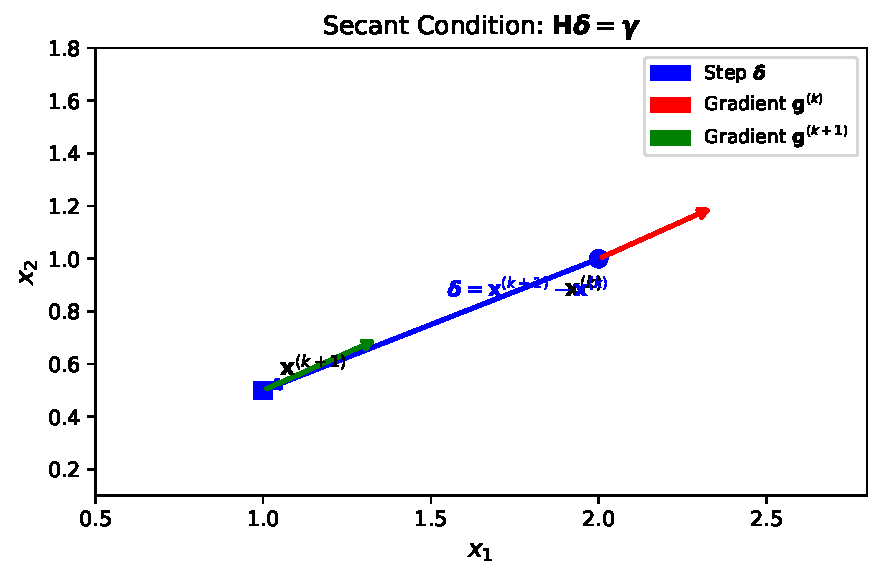
\includegraphics[width=\textwidth]{fig_bfgs_update.pdf}
      {\scriptsize The secant condition $\mathbf{H}\deltabf = \gammabf$ ensures
       the Hessian approximation is consistent with observed gradient changes.}
    \end{column}
  \end{columns}
\end{frame}

\begin{frame}[fragile]{BFGS: Python Implementation}
\begin{lstlisting}[caption={BFGS quasi-Newton method in Python}]
import numpy as np
from numpy.linalg import norm

def bfgs(f, grad_f, x0, eps=1e-8, max_iter=200):
    """BFGS quasi-Newton minimization (NumPy implementation)."""
    x = np.array(x0, dtype=float)
    n = len(x)
    Q = np.eye(n)          # initial inverse Hessian approx = I
    history = [f(x)]

    for _ in range(max_iter):
        g = grad_f(x)
        if norm(g) < eps:
            break
        d = -Q @ g         # descent direction

        # Backtracking line search (Armijo condition)
        alpha, c1 = 1.0, 1e-4
        for _ in range(50):
            if f(x + alpha*d) <= f(x) + c1*alpha*(g @ d):
                break
            alpha *= 0.5

        x_new = x + alpha * d
        g_new = grad_f(x_new)
        delta = x_new - x              # s in standard notation
        gamma = g_new - g              # y in standard notation
        dg = delta @ gamma

        if abs(dg) > 1e-10:            # curvature condition
            rho = 1.0 / dg
            A = np.eye(n) - rho * np.outer(delta, gamma)
            B = np.eye(n) - rho * np.outer(gamma, delta)
            Q = A @ Q @ B + rho * np.outer(delta, delta)  # BFGS update

        x = x_new
        history.append(f(x))
    return x, history

# Compare BFGS with scipy.optimize.minimize
from scipy.optimize import minimize
result = minimize(lambda x: (1-x[0])**2 + 100*(x[1]-x[0]**2)**2,  # Rosenbrock
                  x0=[-1.5, 1.0], method='BFGS',
                  jac=lambda x: np.array([-2*(1-x[0])-400*x[0]*(x[1]-x[0]**2),
                                           200*(x[1]-x[0]**2)]))
print(f"scipy BFGS minimum: {result.x}")      # -> [1. 1.]
print(f"Function evals:     {result.njev}")
\end{lstlisting}
\end{frame}

\begin{frame}[allowframebreaks]{SR1 Update}
  \begin{block}{Symmetric Rank-1 (SR1) Update (Eq.\ 6.26)}
    \[
      \mathbf{Q}^{(k+1)} = \mathbf{Q}^{(k)}
        + \frac{\left(\deltabf - \mathbf{Q}^{(k)}\gammabf\right)
                \left(\deltabf - \mathbf{Q}^{(k)}\gammabf\right)^\top}
               {\left(\deltabf - \mathbf{Q}^{(k)}\gammabf\right)^\top\gammabf}
    \]
  \end{block}

  \begin{columns}[T]
    \begin{column}{0.50\textwidth}
      \begin{block}{SR1 Properties}
        \begin{itemize}
          \item \textbf{Rank-1} update (simpler than BFGS)
          \item Does \emph{not} guarantee positive definiteness
          \item Can be useful when BFGS's rank-2 update
            is too restrictive
          \item Better at capturing non-convex structure
          \item Used in some trust-region frameworks
        \end{itemize}
      \end{block}
    \end{column}
    \begin{column}{0.48\textwidth}
      \begin{alertblock}{When SR1 is Undefined}
        The update is undefined (division by zero) when:
        \[
          \left(\deltabf - \mathbf{Q}^{(k)}\gammabf\right)^\top\gammabf \approx 0
        \]
        In practice: skip the update if the denominator is below a threshold.
      \end{alertblock}
    \end{column}
  \end{columns}

  \framebreak

  \begin{block}{Comparison of Quasi-Newton Update Rules}
    \centering
    \small
    \begin{tabular}{lccccc}
      \toprule
      Method & Rank & Always PD & Inexact LS & Memory & Convergence \\
      \midrule
      SR1   & 1 & No  & Good  & $O(n^2)$ & superlinear \\
      DFP   & 2 & Yes & Poor  & $O(n^2)$ & superlinear \\
      BFGS  & 2 & Yes & Excellent & $O(n^2)$ & superlinear \\
      L-BFGS & 2 & Yes & Good & $O(mn)$ & superlinear \\
      \bottomrule
    \end{tabular}
    \\[4pt]
    {\scriptsize PD = positive definite; LS = line search; $m$ = history size}
  \end{block}

  \centering
  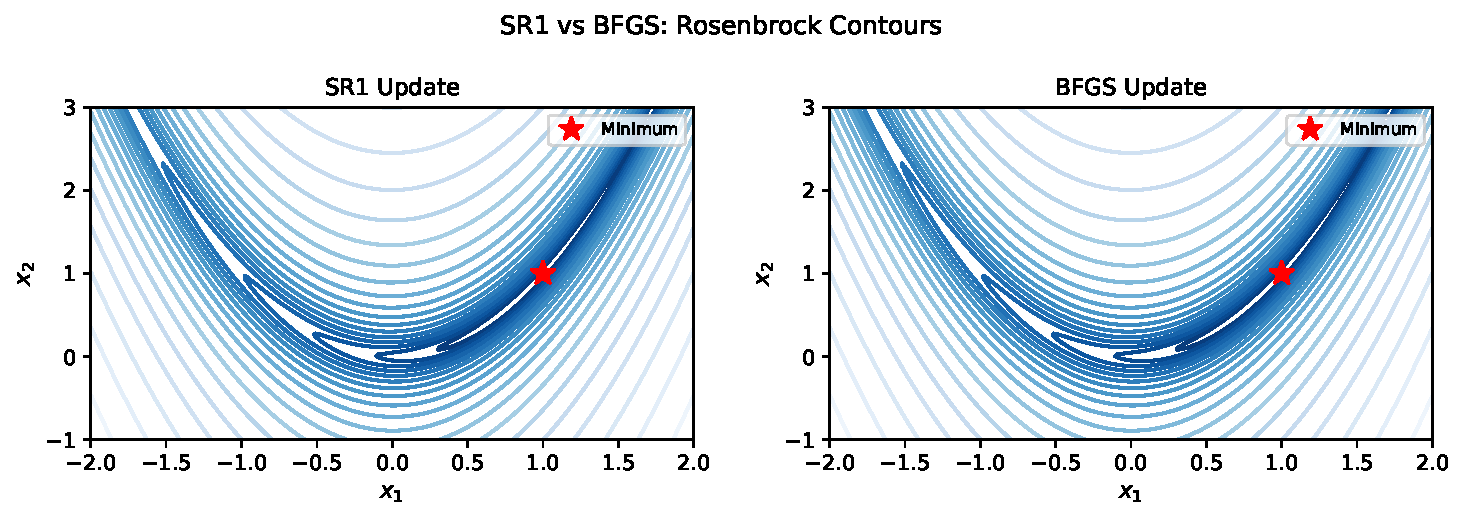
\includegraphics[width=0.55\textwidth]{fig_sr1_vs_bfgs.pdf}
  \\{\scriptsize Contour plots of the Rosenbrock function. Both SR1 and BFGS can navigate curved valleys.}
\end{frame}

\begin{frame}[allowframebreaks]{6.5 L-BFGS: Limited-Memory BFGS}
  \begin{block}{Motivation}
    BFGS stores and updates an $n\times n$ matrix, costing $O(n^2)$ memory.
    For $n = 10^6$, storing $\mathbf{Q}$ is infeasible.
    \textbf{L-BFGS} stores only the last $m$ pairs $\{(\deltabf^{(i)}, \gammabf^{(i)})\}$
    to implicitly approximate the product $\mathbf{Q}\gbf$.
  \end{block}

  \begin{block}{L-BFGS: Two-Loop Recursion (Alg.\ 6.7)}
    \textbf{Backward pass} (compute $\{\alpha^{(i)}\}$, $i = m$ down to $1$):
    \[
      \alpha^{(i)} = \frac{\left(\deltabf^{(i)}\right)^\top\mathbf{q}^{(i)}}
                          {\left(\deltabf^{(i)}\right)^\top\gammabf^{(i)}},
      \qquad
      \mathbf{q}^{(i-1)} = \mathbf{q}^{(i)} - \alpha^{(i)}\gammabf^{(i)}
    \]
    Starting with $\mathbf{q}^{(m)} = \nabla f(\xbf)$.

    \medskip\textbf{Initial scaling:}
    \[
      \mathbf{z}^{(0)} = \frac{\left(\deltabf^{(m)}\right)^\top\gammabf^{(m)}}
                              {\left(\gammabf^{(m)}\right)^\top\gammabf^{(m)}}\,\mathbf{q}^{(0)}
    \]

    \textbf{Forward pass} (compute $\{\mathbf{z}^{(i)}\}$, $i = 1$ to $m$):
    \[
      \mathbf{z}^{(i)} = \mathbf{z}^{(i-1)} + \deltabf^{(i)}
        \left(\alpha^{(i)} - \frac{\left(\gammabf^{(i)}\right)^\top\mathbf{z}^{(i-1)}}
                                  {\left(\deltabf^{(i)}\right)^\top\gammabf^{(i)}}\right)
    \]
    \textbf{Descent direction:} $\mathbf{d} = -\mathbf{z}^{(m)}$
  \end{block}

  \framebreak

  \begin{columns}[T]
    \begin{column}{0.50\textwidth}
      \begin{block}{L-BFGS Algorithm Summary}
        \begin{enumerate}
          \item Initialize: empty history, $\xbf^{(1)}$
          \item Compute $\gbf = \nabla f(\xbf)$
          \item If history empty: $\mathbf{d} = -\gbf$ (steepest descent)
          \item Else: compute $\mathbf{d}$ via two-loop recursion
          \item Line search: find $\alpha^*$
          \item Update: $\xbf \leftarrow \xbf + \alpha^*\mathbf{d}$
          \item Store new $(\deltabf, \gammabf)$; drop oldest if history $> m$
        \end{enumerate}
      \end{block}
      \begin{block}{Memory Comparison}
        \begin{tabular}{ll}
          \toprule
          Method & Memory \\
          \midrule
          BFGS    & $O(n^2)$ \\
          L-BFGS  & $O(mn)$ \\
          \bottomrule
        \end{tabular}
        \\[2pt]
        {\scriptsize Typical: $m = 3$--$20$}
      \end{block}
    \end{column}
    \begin{column}{0.48\textwidth}
      \centering
      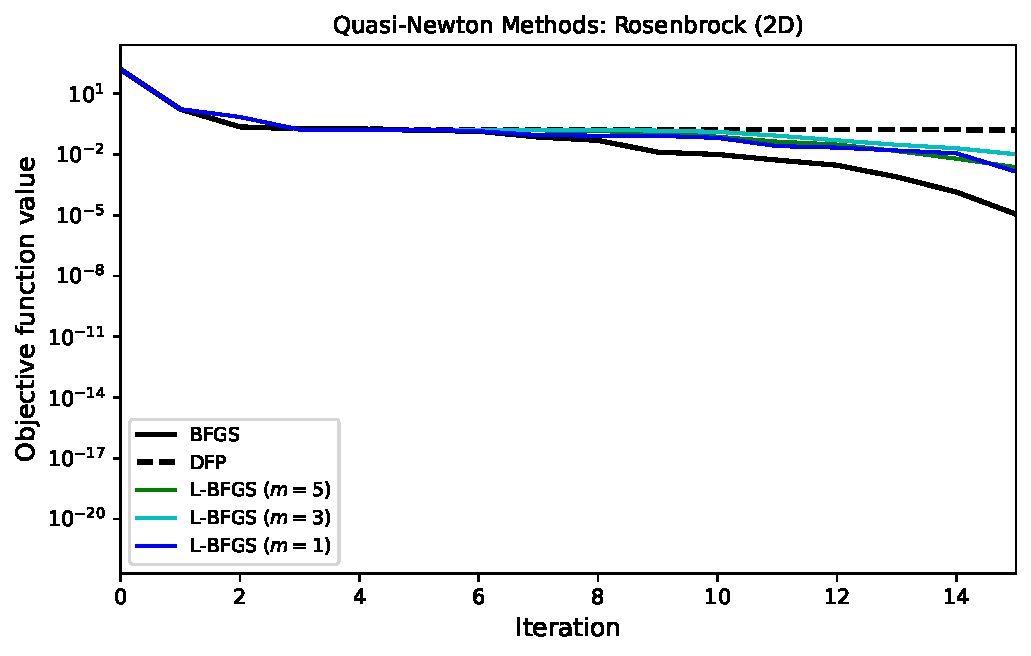
\includegraphics[width=\textwidth]{fig_quasi_newton_comparison.pdf}
      {\scriptsize DFP, BFGS, and L-BFGS variants compared on the 2D Rosenbrock function.
       Larger history $m$ approaches BFGS performance.}
    \end{column}
  \end{columns}
\end{frame}

\begin{frame}[fragile]{L-BFGS: Python Implementation}
\begin{lstlisting}[caption={L-BFGS with two-loop recursion in Python}]
import numpy as np
from collections import deque

def lbfgs(f, grad_f, x0, m=5, eps=1e-8, max_iter=200):
    """L-BFGS quasi-Newton minimization."""
    x = np.array(x0, dtype=float)
    deltas = deque(maxlen=m)    # step differences s_i
    gammas = deque(maxlen=m)    # gradient differences y_i
    history = [f(x)]

    for _ in range(max_iter):
        g = grad_f(x)
        if np.linalg.norm(g) < eps:
            break

        # ---- Two-loop recursion ----
        q = g.copy()
        alphas = []
        for dk, yk in zip(reversed(deltas), reversed(gammas)):
            rho_k = 1.0 / (dk @ yk + 1e-15)
            a = rho_k * (dk @ q)
            q = q - a * yk
            alphas.append((a, rho_k, dk, yk))
        alphas.reverse()

        # Initial scaling
        if deltas:
            dm, ym = deltas[-1], gammas[-1]
            scale = (dm @ ym) / (ym @ ym + 1e-15)
        else:
            scale = 1.0
        z = scale * q

        for (a, rho_k, dk, yk) in alphas:
            beta = rho_k * (yk @ z)
            z = z + dk * (a - beta)
        d = -z
        # ---- End two-loop ----

        # Backtracking line search
        alpha = 1.0
        for _ in range(50):
            if f(x + alpha*d) <= f(x) + 1e-4*alpha*(g @ d):
                break
            alpha *= 0.5

        x_new = x + alpha * d
        g_new = grad_f(x_new)
        deltas.append(x_new - x)
        gammas.append(g_new - g)
        x = x_new
        history.append(f(x))
    return x, history

# SciPy equivalent (uses L-BFGS-B):
from scipy.optimize import minimize
res = minimize(lambda x: (1-x[0])**2 + 100*(x[1]-x[0]**2)**2,
               [-1.5, 1.0], method='L-BFGS-B',
               jac=lambda x: np.array([-2*(1-x[0])-400*x[0]*(x[1]-x[0]**2),
                                        200*(x[1]-x[0]**2)]))
print(f"L-BFGS-B: {res.x}")   # -> [1. 1.]
\end{lstlisting}
\end{frame}

\begin{frame}{Quasi-Newton Methods: Full Comparison}
  \begin{columns}[T]
    \begin{column}{0.48\textwidth}
      \centering
      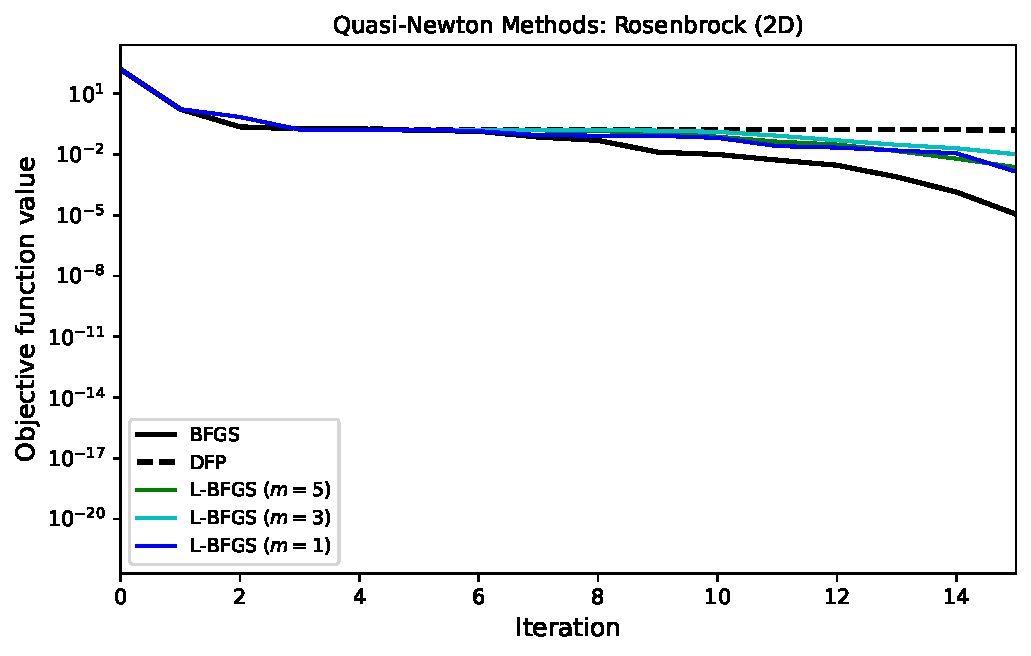
\includegraphics[width=\textwidth]{fig_quasi_newton_comparison.pdf}
      {\scriptsize Objective function vs.\ iteration for BFGS, DFP, and L-BFGS
       variants ($m = 1, 3, 5$) on 2D Rosenbrock. L-BFGS approaches BFGS as $m$ grows.}
    \end{column}
    \begin{column}{0.50\textwidth}
      \begin{block}{Key Observations}
        \begin{itemize}
          \item BFGS and DFP often perform similarly on well-conditioned problems
          \item BFGS outperforms DFP with \emph{inexact} line search
          \item L-BFGS($m=1$) is weakest; L-BFGS($m \geq 5$) nearly matches BFGS
          \item L-BFGS is the \textbf{method of choice for large-scale} problems
            (e.g.\ deep learning, PDE-constrained optimization)
        \end{itemize}
      \end{block}
      \begin{block}{When to Use Which}
        \begin{tabular}{ll}
          \toprule
          Scenario & Method \\
          \midrule
          $n \leq 10^3$, cheap $\Hbf$ & Newton \\
          $n \leq 10^4$, medium & BFGS \\
          $n \geq 10^5$, large-scale & L-BFGS \\
          Nonlinear least squares & LM \\
          \bottomrule
        \end{tabular}
      \end{block}
    \end{column}
  \end{columns}
\end{frame}

% ══════════════════════════════════════════════════════════════
\section{Summary \& Exercises}
% ══════════════════════════════════════════════════════════════

\begin{frame}{6.6 Summary}
  \begin{block}{Chapter Summary}
    \begin{itemize}
      \item \textbf{Second-order information} (Hessian) enables quadratic local
        models that directly yield the optimal step size.
      \item \textbf{Newton's method} uses $\xbf^{(k+1)} = \xbf^{(k)} - \Hbf^{-1}\gbf$.
        Converges quadratically near a minimum; requires positive definite $\Hbf$.
      \item \textbf{Secant method} approximates $f''$ from two gradient evaluations,
        avoiding explicit second derivatives (univariate).
      \item \textbf{Levenberg-Marquardt} interpolates between gradient descent
        ($\delta$ large) and Newton ($\delta$ small), adapting $\delta$ based on
        whether the step was accepted.
      \item \textbf{LM for sum of squares} replaces the Hessian with the
        outer product $\mathbf{J}^\top\mathbf{J}$ (always PSD), requiring only
        first derivatives.
      \item \textbf{Quasi-Newton methods} (DFP, BFGS, L-BFGS) approximate the
        inverse Hessian from gradient differences, achieving superlinear convergence
        without computing $\Hbf$.
      \item \textbf{L-BFGS} reduces memory from $O(n^2)$ to $O(mn)$ by storing
        only the last $m$ step/gradient pairs.
    \end{itemize}
  \end{block}
\end{frame}

\begin{frame}{Method Family Tree}
  \centering
  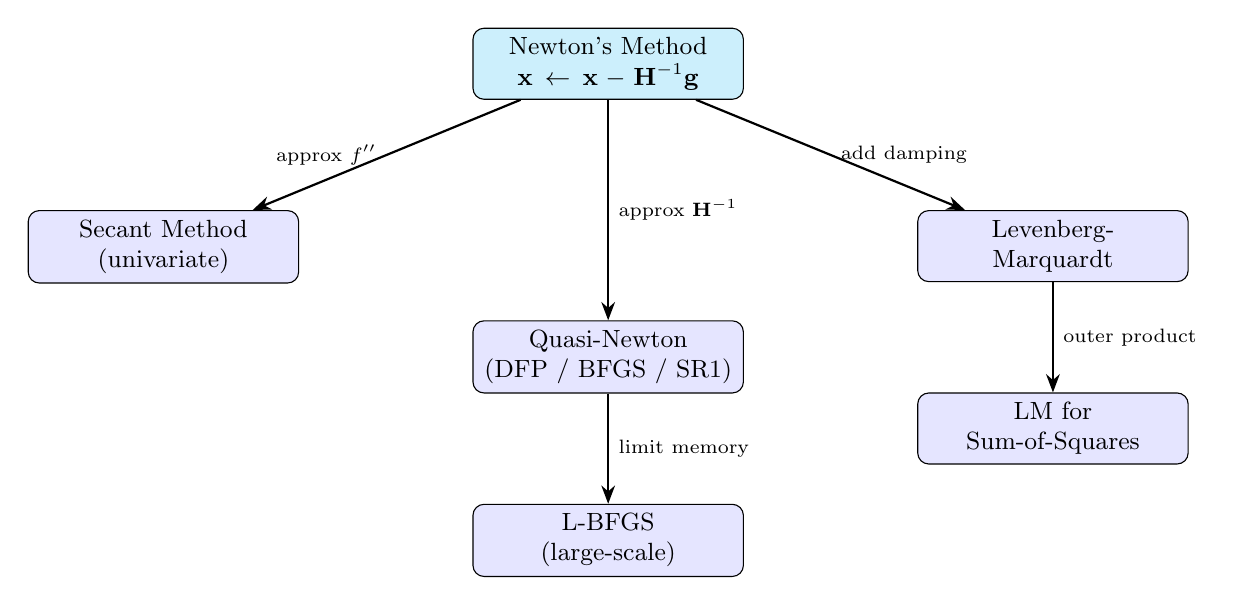
\begin{tikzpicture}[
    node distance=1.4cm and 2.2cm,
    box/.style={draw, rounded corners, fill=blue!10, text width=3.2cm, align=center,
                font=\small, minimum height=0.75cm},
    topbox/.style={draw, rounded corners, fill=cyan!20, text width=3.2cm, align=center,
                font=\small, minimum height=0.75cm},
    arr/.style={-{Stealth}, thick}
  ]
    \node[topbox] (newton) {Newton's Method \\ \small $\mathbf{x} \leftarrow \mathbf{x} - \mathbf{H}^{-1}\mathbf{g}$};
    \node[box, below left=of newton]  (secant)  {Secant Method \\ \small (univariate)};
    \node[box, below right=of newton] (lm)      {Levenberg- \\ Marquardt};
    \node[box, below=2.8cm of newton] (qn)      {Quasi-Newton \\ \small (DFP / BFGS / SR1)};
    \node[box, below=of qn]           (lbfgs)   {L-BFGS \\ \small (large-scale)};
    \node[box, below=of lm]           (lmsos)   {LM for \\ Sum-of-Squares};

    \draw[arr] (newton) -- node[midway,left,font=\scriptsize]{approx $f''$} (secant);
    \draw[arr] (newton) -- node[midway,right,font=\scriptsize]{add damping} (lm);
    \draw[arr] (newton) -- node[midway,right,font=\scriptsize]{approx $\mathbf{H}^{-1}$} (qn);
    \draw[arr] (qn)     -- node[midway,right,font=\scriptsize]{limit memory} (lbfgs);
    \draw[arr] (lm)     -- node[midway,right,font=\scriptsize]{outer product} (lmsos);
  \end{tikzpicture}
\end{frame}

\begin{frame}{6.7 Selected Exercises}
  \begin{block}{Exercise 6.1}
    \textbf{Q:} What advantage does second-order information provide about convergence
    that first-order information lacks?

    \medskip\textbf{A:} Second-order information can \emph{guarantee} that one is at a local
    minimum (via positive definiteness of the Hessian), whereas a gradient of zero
    is necessary but insufficient to guarantee local optimality.
  \end{block}

  \begin{block}{Exercise 6.9}
    \textbf{Q:} Starting from the origin, apply one step of Newton's method to
    $f(\xbf) = (x_1+1)^2 + (x_2+3)^2 + 4$.

    \medskip\textbf{A:} $\nabla f = [2(x_1+1),\,2(x_2+3)]^\top = [2,\,6]^\top$,
    $\Hbf = 2\Ibf$.
    \[
      \xbf^{(2)} = [0,0]^\top - (2\Ibf)^{-1}[2,6]^\top = [-1,\,-3]^\top = \xbf^*
    \]
    Converges in one step since $f$ is quadratic.
  \end{block}

  \begin{block}{Exercise 6.7}
    \textbf{Q:} What is the advantage of a quasi-Newton method over Newton's method?

    \medskip\textbf{A:} It does not need computation of the Hessian entries and
    hence does not require solving a linear system at each iteration using the
    exact Hessian.
  \end{block}
\end{frame}

\begin{frame}{Selected Exercises (continued)}
  \begin{block}{Exercise 6.2}
    \textbf{Q:} When finding roots in one dimension, when would we use Newton's
    method instead of the bisection method?

    \medskip\textbf{A:} Newton's method is preferred when:
    \begin{itemize}
      \item The derivative is available and cheap to compute
      \item High accuracy is needed quickly (quadratic vs.\ linear convergence)
      \item The starting point is already close to the root
    \end{itemize}
    Bisection is preferred when derivatives are unavailable or when you need
    guaranteed convergence with bracketing.
  \end{block}

  \begin{block}{Exercise 6.8}
    \textbf{Q:} Give an example where the BFGS update does not exist. What would you do?

    \medskip\textbf{A:} The BFGS update does not exist when
    $\deltabf^\top\gammabf \approx 0$ (curvature condition fails).
    In that case, simply \textbf{skip the update} and keep the current
    inverse Hessian approximation for that iteration.
  \end{block}

  \begin{block}{Exercise 6.6}
    \textbf{Q:} Give a sequence $\{x^{(k)}\}$ with decreasing $f$ that does not converge.

    \medskip\textbf{A:} $x^{(k+1)} = x^{(k)}/2$ starting from $x^{(1)} = -1$ on
    $f(x) = x^2 - x$. Values decrease but the sequence converges to $x = 0$,
    which is not the minimizer $x^* = 0.5$.
  \end{block}
\end{frame}

\begin{frame}{Quick Reference: Second-Order Methods}
  \centering
  \small
  \begin{tabular}{p{2.8cm}p{4.5cm}p{2.5cm}p{2.0cm}}
    \toprule
    \textbf{Method} & \textbf{Update Rule} & \textbf{Requirements} & \textbf{Convergence} \\
    \midrule
    Newton's Method &
    $\xbf \leftarrow \xbf - \Hbf^{-1}\gbf$ &
    $\nabla f$, $\nabla^2 f$ &
    Quadratic \\[4pt]
    Secant Method &
    $x \leftarrow x - \tfrac{x - x_\text{prev}}{g - g_\text{prev}}g$ &
    $f'$ only &
    Superlinear \\[4pt]
    Levenberg-Marquardt &
    $\xbf \leftarrow \xbf - (\Hbf + \delta D)^{-1}\gbf$ &
    $\nabla f$, $\nabla^2 f$ &
    Adaptive \\[4pt]
    LM Sum of Squares &
    $\xbf \leftarrow \xbf - (\mathbf{J}^\top\mathbf{J} + \delta D)^{-1}\mathbf{J}^\top\mathbf{r}$ &
    $\mathbf{J}$ only &
    Adaptive \\[4pt]
    DFP &
    $\mathbf{Q} \leftarrow \mathbf{Q} - \tfrac{\mathbf{Q}\gammabf\gammabf^\top\mathbf{Q}}{\gammabf^\top\mathbf{Q}\gammabf} + \tfrac{\deltabf\deltabf^\top}{\deltabf^\top\gammabf}$ &
    $\nabla f$ only &
    Superlinear \\[4pt]
    BFGS &
    $\mathbf{Q} \leftarrow (\Ibf - \rho\deltabf\gammabf^\top)\mathbf{Q}(\Ibf - \rho\gammabf\deltabf^\top) + \rho\deltabf\deltabf^\top$ &
    $\nabla f$ only &
    Superlinear \\[4pt]
    L-BFGS &
    Two-loop recursion with $m$ history pairs &
    $\nabla f$ only &
    Superlinear \\
    \bottomrule
  \end{tabular}
  \vspace{6pt}
  {\scriptsize $D = \mathrm{diag}(\Hbf)$ or $\Ibf$; $\rho = 1/(\deltabf^\top\gammabf)$}
\end{frame}

\end{document}
